\chapter{State of the art}
\minitoc
\newpage

\setcounter{secnumdepth}{0} % Set the section counter to 0 so next section is not counted in toc
% ----------------------- Introduction ----------------------- %
\section{Introduction}
This chapter presents and studies various concepts essential to modernizing Navoy's AI travel platform, with particular emphasis on network engineering principles, cloud infrastructure design, and network security practices.
I will discuss the most used tools in the market as well as which ones I settled on after making comparative studies to ensure the best fit for a scalable, network-optimized travel technology platform across multiple cloud providers.

\setcounter{secnumdepth}{2} % Resume counting the sections for the toc with a depth of 2 (Sections and sub-sections)
% ----------------------------------- SECTIONS (v) ----------------------------------- %
% ----------------------- DevSecOps ----------------------- %
\section{DevSecOps}

\subsection{Definition}
DevSecOps stands for development, security, and operations. It's an approach to culture, automation, and platform design that integrates security as a shared responsibility throughout the entire IT lifecycle \cite{redhat-devsecops}. Unlike traditional approaches where security is treated as a separate phase, DevSecOps embeds security considerations from the initial design through deployment and maintenance. This approach is particularly crucial for travel technology platforms like Navoy's, where sensitive user data, payment information, and booking details must be protected throughout the entire development and deployment process.

The core addittion of DevSecOps over DevOps is "security as code," meaning that security policies, compliance checks, and vulnerability assessments are automated and integrated directly into CI/CD pipelines. This ensures that security is not an afterthought but a fundamental aspect of the development process, enabling faster and more secure releases.

\subsection{DevSecOps Lifecycle}
\begin{figure}[H]
    \centering
    \makebox[\textwidth]{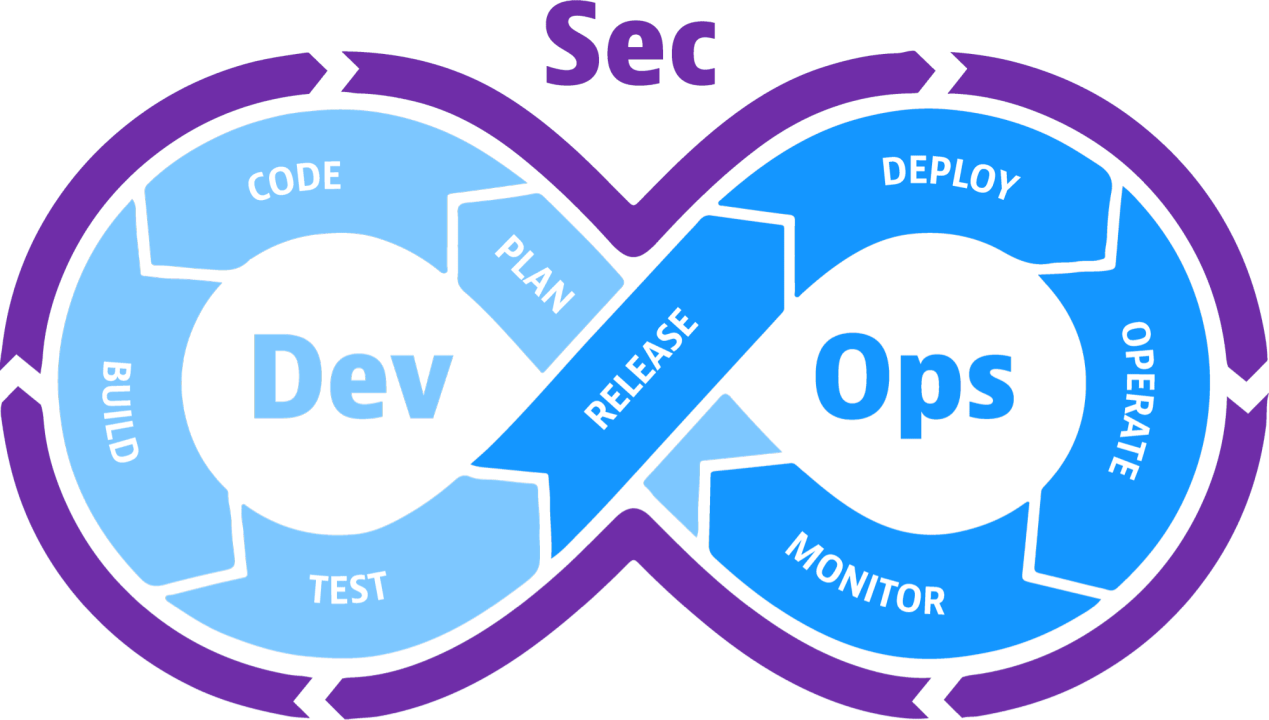
\includegraphics[width=8cm]{src/assets/images/devsecops-lifecycle.png}}
    \caption{DevSecOps Lifecycle}
    \label{fig:devops-lifecycle}
\end{figure}

The DevSecOps lifecycle consists of several key phases that integrate security seamlessly into development operations:

\begin{itemize}
    \item \textbf{Plan}: Security requirements and threat modeling are incorporated during the planning phase
    \item \textbf{Code}: Secure coding practices and static application security testing (SAST) are applied
    \item \textbf{Build}: Security scanning and dependency vulnerability checks are automated
    \item \textbf{Test}: Dynamic application security testing (DAST) and penetration testing are performed
    \item \textbf{Deploy}: Infrastructure security scans and compliance checks are executed
    \item \textbf{Monitor}: Continuous security monitoring and incident response are maintained
\end{itemize}

For Navoy's AI travel platform, this lifecycle ensures that security vulnerabilities are caught early, reducing the risk of exposing sensitive travel data and maintaining compliance with data protection regulations.

\subsection{Container Security}
Container security is a critical aspect of DevSecOps, especially when deploying microservices architectures. It involves securing the entire container lifecycle from image creation to runtime.

\subsubsection*{What is container security?}
Container security is the process of safeguarding containerized applications from malware and other vulnerabilities \cite{redhat-container-security}. This includes securing container images, the container runtime, and the orchestration platform. Key aspects include vulnerability scanning of base images, implementing least-privilege access controls, and continuous monitoring of container behavior.

\subsubsection*{Security scanning in CI/CD}
CI/CD security is the distribution of security practices and measures throughout the continuous integration and continuous delivery (CI/CD) pipeline \cite{paloalto-cicd-security}. This includes scanning container images for known vulnerabilities, checking dependencies for security issues, and performing static code analysis. For Navoy's platform, this ensures that no vulnerable components are deployed to production, maintaining the security of the travel booking system.

\subsection{Infrastructure as Code (IaC) Security}

\subsubsection*{What is IaC?}
Infrastructure as code (IaC) is the ability to provision and support your computing infrastructure using code instead of manual processes and settings. Any application environment requires many infrastructure components like operating systems, database connections, and storage. Developers have to regularly set up, update, and maintain the infrastructure to develop, test, and deploy applications \cite{aws-iac}.

\subsubsection*{Importance of IaC}
IaC ensures high availability by enabling rapid infrastructure replication and scaling across multiple regions. It enhances disaster recovery capabilities by allowing infrastructure to be quickly recreated from code in case of failures, ensuring business continuity for critical systems like Navoy's platform. Additionally, IaC reduces human error, improves consistency, and enables faster deployment cycles across multiple cloud providers.

\subsubsection*{IaC Security Best Practices}
IaC security involves applying security best practices to infrastructure definitions and ensuring cloud resources are configured securely by default. This includes scanning IaC templates for misconfigurations, implementing policy as code, and maintaining compliance with security standards throughout the provisioning process.

% ----------------------- AI Technologies ----------------------- %
\section{AI Technologies for Trip Generation}

\subsection{Large Language Models (LLMs)}
Large Language Models (LLMs) are advanced deep learning models trained on vast corpora of text data to understand and generate human-like language. Architecturally, most state-of-the-art LLMs are based on the Transformer model \cite{vaswani2017attention}, which leverages self-attention mechanisms to capture complex dependencies in text. These models are pre-trained on large-scale datasets and then fine-tuned for specific tasks, enabling them to perform a wide range of natural language processing (NLP) applications such as text generation, summarization, translation, and question answering \cite{brown2020language, touvron2023llama}.

The core technology powering Navoy's AI-driven trip generation capabilities is the LLM. These models can interpret natural language inputs from users describing their travel preferences and generate personalized itineraries with contextual recommendations for destinations, activities, accommodations, and dining options. The ability of LLMs to process unstructured user requests and transform them into structured, actionable travel plans is a significant advancement in AI-driven travel technology \cite{bommasani2021opportunities}.

Recent research highlights the effectiveness of LLMs in understanding context, maintaining coherence over long conversations, and adapting to user-specific requirements \cite{openai2023gpt4, zhao2023survey}. For travel technology platforms like Navoy's, this means LLMs can deliver highly personalized and conversational experiences that align with modern user expectations for AI assistants.

\subsection{Model Selection and Integration}
The choice of LLM provider and integration approach is crucial for maintaining both quality and reliability in AI-powered travel recommendations.

\subsection{AI Models: OpenAI GPT vs Claude}
\renewcommand{\arraystretch}{1.5}
\begin{longtable}{| p{0.2\textwidth} | p{0.38\textwidth} | p{0.38\textwidth} |}
    \caption{Comparative study between OpenAI GPT, Claude, and LiteLLM}                                                                                                                                                                                                                                \\
    \hline
    \rowcolor{primary} \textbf{Provider} & \textbf{OpenAI GPT Models}                                                                                                      & \textbf{Claude (Anthropic)}                                                                                               \\
    \hline
    \endfirsthead

    \multicolumn{3}{c}%
    {{\bfseries \tablename\ \thetable{} -- continued from previous page}}                                                                                                                                                                                                                              \\
    \hline
    \rowcolor{primary} \textbf{Provider} & \textbf{OpenAI GPT Models}                                                                                                      & \textbf{Claude (Anthropic)}                                                                                               \\
    \hline
    \endhead

    \hline \multicolumn{3}{|r|}{{Continued on next page}}                                                                                                                                                                                                                                              \\
    \endfoot

    \hline
    \endlastfoot

    \textbf{Strengths}                   & Excellent at creative itinerary generation, wide knowledge base, and strong reasoning capabilities for complex travel planning. & Superior safety features, detailed explanations, and excellent at handling nuanced travel preferences and constraints.    \\
    \hline
    \textbf{Use Case}                    & Ideal for generating diverse travel options, creative recommendations, and handling multi-destination complex itineraries.      & Perfect for detailed travel planning, safety considerations, and providing comprehensive travel advice with explanations. \\
    \hline
    \textbf{Integration}                 & Direct API integration with reliable performance and extensive documentation.                                                   & Clean API with focus on helpful, harmless, and honest responses ideal for travel recommendations.                         \\
    \hline
\end{longtable}

\subsection{LiteLLM Integration Approach}
\begin{figure}[H]
    \centering
    \makebox[\textwidth]{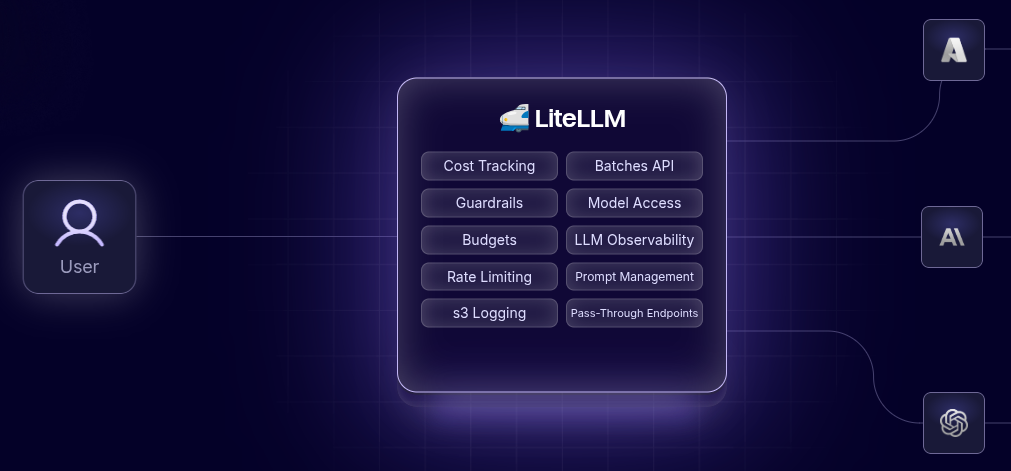
\includegraphics[width=12cm]{src/assets/images/litellm.png}}
    \caption{LiteLLM}
    \label{fig:litellm}
\end{figure}

For Navoy's AI travel platform, I chose to implement LiteLLM as the primary integration solution. According to its official description, LiteLLM is an "LLM Gateway to provide model access, fallbacks and spend tracking across 100+ LLMs. All in the same API"\cite{litellm}. It acts as a proxy service that provides a unified interface to access multiple LLM providers including OpenAI, Anthropic, Google, and others through a single API.

The key advantages of using LiteLLM include enabling model switching without code changes, cost optimization through provider comparison, fallback mechanisms for reliability, and unified monitoring across all models. It serves as a simple drop-in replacement for OpenAI API calls while supporting load balancing, rate limiting, and providing comprehensive logging and analytics.

This approach allows organic access to both OpenAI's GPT models and Claude, providing flexibility to use the best model for specific tasks—GPT for creative itinerary generation and Claude for detailed travel advice—while maintaining a unified codebase and enabling cost optimization through intelligent model routing.

% ----------------------- Cloud Infrastructure and Network Architecture ----------------------- %
\section{Cloud Infrastructure and Network Architecture}

\subsection{Multi-Cloud Network Design}
Modern travel platforms require robust, scalable network infrastructure that can handle global traffic patterns and ensure low-latency access to AI services. The network architecture must support microservices communication, secure data transmission, and efficient traffic routing across multiple cloud regions.

For Navoy's AI travel platform, the network design encompasses VPC architecture, subnet segmentation, load balancing strategies, CDN implementation, and cross-cloud connectivity. This infrastructure supports both the distributed microservices architecture and the AI model serving requirements while maintaining security and performance standards.

\subsection{Network Security and Compliance}
Network security is paramount for travel platforms handling sensitive user data, payment information, and booking details. The architecture must implement defense-in-depth strategies including network segmentation, traffic encryption, DDoS protection, and compliance with international data protection regulations.

The network security framework includes firewall configurations, security groups, network access control lists, VPN gateways for secure connectivity, and monitoring systems for threat detection and response. These components work together to create a comprehensive security posture that protects both infrastructure and application layers.

\subsection{Cloud Providers: Azure vs AWS}
For cloud infrastructure deployment, selecting the right provider and understanding their networking capabilities is crucial for optimal performance and cost management.

\renewcommand{\arraystretch}{1.5}%
\begin{longtable}{| p{0.2\textwidth} | p{0.38\textwidth} | p{0.38\textwidth} |}
    \caption{Comparative study between Microsoft Azure and Amazon AWS}                                                                                                                                                                                                                            \\
    \hline
    \rowcolor{primary} \textbf{Aspect} & \textbf{Microsoft Azure}                                                                                                             & \textbf{Amazon AWS}                                                                                               \\
    \hline
    \endfirsthead

    \multicolumn{3}{c}%
    {{\bfseries \tablename\ \thetable{} -- continued from previous page}}                                                                                                                                                                                                                         \\
    \hline
    \rowcolor{primary} \textbf{Aspect} & \textbf{Microsoft Azure}                                                                                                             & \textbf{Amazon AWS}                                                                                               \\
    \hline
    \endhead

    \hline \multicolumn{3}{|r|}{{Continued on next page}}                                                                                                                                                                                                                                         \\
    \endfoot

    \hline
    \endlastfoot

    \textbf{Network Architecture}      & Virtual Networks (VNets) with advanced peering, ExpressRoute for hybrid connectivity, and Traffic Manager for global load balancing. & VPC with advanced routing, Direct Connect for dedicated connectivity, and Route 53 for DNS-based traffic routing. \\
    \hline
    \textbf{Global Infrastructure}     & 60+ regions with strong presence in Europe and integration with Microsoft ecosystem.                                                 & 80+ regions with extensive global coverage and mature edge locations for CDN services.                            \\
    \hline
    \textbf{Network Security}          & Azure Firewall, Network Security Groups, and DDoS Protection with integrated Microsoft security ecosystem.                           & Security Groups, NACLs, AWS WAF, and comprehensive DDoS protection with CloudFlare integration.                   \\
    \hline
    \textbf{Load Balancing}            & Application Gateway, Load Balancer, and Front Door for global load balancing with SSL termination.                                   & Application Load Balancer, Network Load Balancer, and CloudFront for global content delivery.                     \\
    \hline
    \textbf{Networking Costs}          & Competitive pricing for data transfer within regions, free ingress traffic.                                                          & Mature pricing model with reserved capacity options and data transfer optimization features.                      \\
    \hline
\end{longtable}

For Navoy's platform, I implemented a multi-cloud strategy utilizing both Azure and AWS to leverage the strengths of each provider. Azure provides excellent integration with development tools and cost-effective European operations, while AWS offers superior global reach and mature AI/ML services for the trip generation components.

\subsection{Network Monitoring: Prometheus vs Azure Monitor vs CloudWatch}
Network monitoring and observability are critical for maintaining the performance and reliability of distributed travel platforms across multiple cloud environments.

\renewcommand{\arraystretch}{1.5}%
\begin{longtable}{| p{0.2\textwidth} | p{0.38\textwidth} | p{0.38\textwidth} |}
    \caption{Comparative study of Network Monitoring Solutions}                                                                                                                                                                                                                                         \\
    \hline
    \rowcolor{primary} \textbf{Solution} & \textbf{Network Monitoring Capabilities}                                                                                                     & \textbf{Integration and Scalability}                                                                          \\
    \hline
    \endfirsthead

    \multicolumn{3}{c}%
    {{\bfseries \tablename\ \thetable{} -- continued from previous page}}                                                                                                                                                                                                                               \\
    \hline
    \rowcolor{primary} \textbf{Solution} & \textbf{Network Monitoring Capabilities}                                                                                                     & \textbf{Integration and Scalability}                                                                          \\
    \hline
    \endhead

    \hline \multicolumn{3}{|r|}{{Continued on next page}}                                                                                                                                                                                                                                               \\
    \endfoot

    \hline
    \endlastfoot

    \textbf{Prometheus}                  & Open-source metrics collection with custom network exporters, supports multi-cloud environments, and provides flexible querying with PromQL. & Excellent Kubernetes integration, supports federated monitoring across multiple clusters and cloud providers. \\
    \hline
    \textbf{Azure Monitor}               & Native Azure network monitoring with Network Watcher, VNet flow logs, and Application Gateway analytics.                                     & Deep integration with Azure services, supports hybrid monitoring with on-premises connectivity insights.      \\
    \hline
    \textbf{AWS CloudWatch}              & Comprehensive AWS network metrics, VPC Flow Logs analysis, and X-Ray for distributed tracing across network boundaries.                      & Native AWS integration, supports cross-region monitoring and custom network performance dashboards.           \\
    \hline
\end{longtable}

For Navoy's multi-cloud architecture, I implemented a hybrid monitoring approach using Prometheus for cross-cloud metrics aggregation, complemented by native cloud monitoring services for cloud-specific network insights and detailed traffic analysis.

% ----------------------- Comparative Analysis ----------------------- %
\section{Comparative Analysis}
In order to modernize Navoy's AI travel platform and implement proper DevSecOps practices, I need a wide range of tools that deal with the following areas: version control, container orchestration, infrastructure as code, and automated testing. For that, I conducted a comparative study on some of the tools the market provides.

\subsection{Version Control: GitLab vs GitHub}
Modern DevSecOps relies on robust version control for collaboration and code management. GitLab and GitHub are leading platforms based on Git, supporting change tracking, branching, and team workflows. While both offer similar core features—like pull/merge requests and code review—they differ in their approach to DevOps integration.

The table below compares their version control and DevSecOps integration:

\renewcommand{\arraystretch}{1.5}%
\begin{longtable}{| p{0.2\textwidth} | p{0.38\textwidth} | p{0.38\textwidth} |}
    \caption{Comparative study between GitLab and GitHub}                                                                                                                                                                                                 \\
    \hline
    \rowcolor{primary} \textbf{Aspect} & \textbf{GitLab}                                                                                             & \textbf{GitHub}                                                                                    \\
    \hline
    \endfirsthead

    \multicolumn{3}{c}%
    {{\bfseries \tablename\ \thetable{} -- continued from previous page}}                                                                                                                                                                                 \\
    \hline
    \rowcolor{primary} \textbf{Aspect} & \textbf{GitLab}                                                                                             & \textbf{GitHub}                                                                                    \\
    \hline
    \endhead

    \hline \multicolumn{3}{|r|}{{Continued on next page}}                                                                                                                                                                                                 \\
    \endfoot

    \hline
    \endlastfoot

    \textbf{Version Control Features}  & Distributed version control with Git, merge requests, integrated code review, and granular access controls. & Distributed version control with Git, pull requests, code review, and fine-grained permissions.    \\
    \hline
    \textbf{DevSecOps Integration}     & Complete DevSecOps platform with built-in SAST, DAST, dependency scanning, and container scanning.          & Requires third-party integrations and GitHub Actions for comprehensive security scanning.          \\
    \hline
    \textbf{CI/CD Capabilities}        & Built-in CI/CD with powerful pipelines, auto-scaling runners, and advanced caching.                         & GitHub Actions provides flexible automation but requires more configuration for complex scenarios. \\
    \hline
    \textbf{Self-Hosting}              & Robust self-hosting with GitLab CE/EE, providing complete control over data and infrastructure.             & GitHub Enterprise Server offers limited self-hosting features.                                     \\
    \hline
\end{longtable}

Both platforms excel at version control, but GitLab stands out for its built-in DevSecOps and CI/CD, while GitHub relies more on third-party tools and Actions for automation and security.

For Navoy's platform, I chose GitLab for its integrated security, DevSecOps features, and existing self-hosted setup, ensuring full control over sensitive data and seamless security in the development pipeline.

\subsection{Infrastructure as Code: Terraform vs Pulumi}
Terraform and Pulumi are leading tools for managing cloud infrastructure programmatically. While both enable infrastructure provisioning, they differ in language support, ecosystem maturity, and workflow integration.

\renewcommand{\arraystretch}{1.5}%
\begin{longtable}{| p{0.2\textwidth} | p{0.38\textwidth} | p{0.38\textwidth} |}
    \caption{Comparative study between Terraform and Pulumi}                                                                                                                                                                                                 \\
    \hline
    \rowcolor{primary} \textbf{Aspect} & \textbf{Terraform}                                                                                           & \textbf{Pulumi}                                                                                      \\
    \hline
    \endfirsthead

    \multicolumn{3}{c}%
    {{\bfseries \tablename\ \thetable{} -- continued from previous page}}                                                                                                                                                                                    \\
    \hline
    \rowcolor{primary} \textbf{Aspect} & \textbf{Terraform}                                                                                           & \textbf{Pulumi}                                                                                      \\
    \hline
    \endhead

    \hline \multicolumn{3}{|r|}{{Continued on next page}}                                                                                                                                                                                                    \\
    \endfoot

    \hline
    \endlastfoot

    \textbf{Language Support}          & Uses HCL (HashiCorp Configuration Language) specifically designed for infrastructure provisioning.           & Supports multiple programming languages including TypeScript, Python, Go, and C\#.                   \\
    \hline
    \textbf{State Management}          & Mature state management with remote backends, state locking, and collaborative workflows.                    & Uses state files with managed service for storage by default and additional cloud-based features.    \\
    \hline
    \textbf{Ecosystem \& Maturity}     & Larger ecosystem, extensive provider support, and widespread enterprise adoption. Industry standard for IaC. & Newer but growing rapidly with good provider support and unique testing frameworks.                  \\
    \hline
    \textbf{DevSecOps Integration}     & Integrates well with security scanning tools. Policy as code via Sentinel or Open Policy Agent.              & Native support for policy as code and testing frameworks with good development workflow integration. \\
    \hline
\end{longtable}

For Navoy's infrastructure, I chose Terraform due to its maturity, provider ecosystem, and the team's familiarity with HCL. Its robust state management and industry adoption make it ideal for managing complex, scalable cloud environments.

\subsection{Deployment: Docker Swarm vs Kubernetes}

\subsubsection*{Container Orchestration}
Docker Compose is a tool for defining and running multi-container applications \cite{docker-compose} and whilte it is great for local development and testing, but it is not suitable for production. It lacks high availability, automated failover, rolling updates, and dynamic scaling. Without features like native service discovery, self-healing, or advanced networking, Compose cannot reliably manage complex, distributed applications at scale. Using it in production can result in downtime and manual intervention.

For production, container orchestration is essential. Tools like Kubernetes and Docker Swarm automate deployment, scaling, and management of containers across clusters. Kubernetes stands out for its self-healing, auto-scaling, declarative configuration, and large ecosystem. While Docker Compose can define multi-container apps, it lacks the automation, resilience, and scalability needed for cloud-native workloads. Moving to Kubernetes or a similar orchestrator ensures reliability and maintainability.

Our research led us to compare Docker Swarm and Kubernetes.

\subsubsection*{Docker Swarm vs Kubernetes}
\renewcommand{\arraystretch}{1.5}%
\begin{longtable}{| p{0.2\textwidth} | p{0.38\textwidth} | p{0.38\textwidth} |}
    \caption{Comparative study between Docker Swarm and Kubernetes}                                                                                                                                                                                                                                                                                                           \\
    \hline
    \rowcolor{primary} \textbf{Aspect} & \textbf{Docker Swarm}                                                                                                                                                                                                                                                        & \textbf{Kubernetes}                                   \\
    \hline
    \endfirsthead

    \multicolumn{3}{c}%
    {{\bfseries \tablename\ \thetable{} -- continued from previous page}}                                                                                                                                                                                                                                                                                                     \\
    \hline
    \rowcolor{primary} \textbf{Aspect} & \textbf{Docker Swarm}                                                                                                                                                                                                                                                        & \textbf{Kubernetes}                                   \\
    \hline
    \endhead

    \hline \multicolumn{3}{|r|}{{Continued on next page}}                                                                                                                                                                                                                                                                                                                     \\
    \endfoot

    \hline
    \endlastfoot

    \textbf{Overview}                  & \multicolumn{2}{p{0.76\textwidth}|}{Docker Swarm is a lightweight, easy-to-use orchestration tool with limited offerings compared to Kubernetes. In contrast, Kubernetes is complex but powerful and it provides self-healing and auto-scaling capabilities out of the box.}                                                         \\
    \hline
    \textbf{Advantages}                & \begin{itemize}[leftmargin=*, topsep=0pt, itemsep=1pt, parsep=2pt]
        \item Easy to install and learn
        \item Works with Docker CLI
    \end{itemize}                                                                                                                                                                                                                                                & \begin{itemize}[leftmargin=*, topsep=0pt, itemsep=1pt, parsep=2pt]
        \item Manages large architectures and complex workloads
        \item Self-healing with automatic scaling
        \item Cross-platform support
        \item Large community with Google backing
        \item Industry standard orchestrator
    \end{itemize}                        \\
    \hline
    \textbf{Disadvantages}             & Abandoned by Docker Inc. and no longer maintained.                                                                                                                                                                                                                           & Steep learning curve and requires separate CLI tools. \\
    \hline
\end{longtable}
Therefore, we will be deploying our application stack to Kubernetes since the potential is huge compared to the deprecated Docker Swarm.

\subsection{Automated Testing: Jest vs Playwright}
Automated testing is crucial for DevSecOps pipelines, ensuring code quality and preventing regressions. For Navoy's platform, both unit testing and end-to-end testing are essential.

\renewcommand{\arraystretch}{1.5}%
\begin{longtable}{| p{0.2\textwidth} | p{0.38\textwidth} | p{0.38\textwidth} |}
    \caption{Comparative study between Jest and Playwright}                                                                                                                                                                                                                               \\
    \hline
    \rowcolor{primary} \textbf{Aspect} & \textbf{Jest}                                                                                                                 & \textbf{Playwright}                                                                                              \\
    \hline
    \endfirsthead

    \multicolumn{3}{c}%
    {{\bfseries \tablename\ \thetable{} -- continued from previous page}}                                                                                                                                                                                                                 \\
    \hline
    \rowcolor{primary} \textbf{Aspect} & \textbf{Jest}                                                                                                                 & \textbf{Playwright}                                                                                              \\
    \hline
    \endhead

    \hline \multicolumn{3}{|r|}{{Continued on next page}}                                                                                                                                                                                                                                 \\
    \endfoot

    \hline
    \endlastfoot

    \textbf{Testing Type}              & Unit testing framework for testing components, functions, and modules in isolation. Excels at business logic and API testing. & End-to-end testing framework supporting multiple browsers (Chromium, Firefox, WebKit) for cross-browser testing. \\
    \hline
    \textbf{Performance}               & Fast parallel test execution with built-in mocking and snapshot testing.                                                      & Fast and reliable with automatic waiting, parallel execution, and test isolation.                                \\
    \hline
    \textbf{DevSecOps Integration}     & Seamless CI/CD integration with coverage reports and build failure on threshold violations.                                   & Excellent CI/CD integration with Docker support and automatic screenshot/video capture on failures.              \\
    \hline
    \textbf{Browser Support}           & Focuses on unit testing, can use jsdom for DOM testing.                                                                       & Supports all modern browsers for comprehensive cross-browser testing.                                            \\
    \hline
\end{longtable}

For Navoy's platform, I chose to implement both Jest for comprehensive unit testing of microservices and business logic, and Playwright for end-to-end testing of critical user journeys like trip planning and booking flows. This combination ensures both code quality and user experience validation across multiple browsers.

\subsection{Deployment management: Kubectl vs Helm}
Since we're using Kubernetes, we have the option to deploy our microservices either with Kubectl or with Helm.

\renewcommand{\arraystretch}{1.5}%
\begin{longtable}{| p{0.2\textwidth} | p{0.38\textwidth} | p{0.38\textwidth} |}
    \caption{Comparative study between Kubectl and Helm}                                                                                                                                                                                                                                                      \\
    \hline
    \rowcolor{primary} \textbf{Aspect} & \textbf{Kubectl}                                                                                                                  & \textbf{Helm}                                                                                                                    \\
    \hline
    \endfirsthead

    \multicolumn{3}{c}%
    {{\bfseries \tablename\ \thetable{} -- continued from previous page}}                                                                                                                                                                                                                                     \\
    \hline
    \rowcolor{primary} \textbf{Aspect} & \textbf{Kubectl}                                                                                                                  & \textbf{Helm}                                                                                                                    \\
    \hline
    \endhead

    \hline \multicolumn{3}{|r|}{{Continued on next page}}                                                                                                                                                                                                                                                     \\
    \endfoot

    \hline
    \endlastfoot

    \textbf{Overview}                  & The official Kubernetes command-line tool for running commands against clusters.                                                  & The package manager for Kubernetes applications.                                                                                 \\
    \hline
    \textbf{Capabilities}              & Deploy applications, manage cluster resources, view logs, and advanced features like node tainting and load balancing strategies. & Define, install, and upgrade complex Kubernetes applications with templates to avoid code duplication between similar resources. \\
    \hline
\end{longtable}
Thoroughly studying our use case, we agreed to create a uniform Helm package to ship our microservices.
We also deemed it necessary to have some common configuration that we simply apply with Kubectl such as Ingress rules or letsencrypt certificates for convenience purposes and due to the lack of time.
% ----------------------------------- SECTIONS (^) ----------------------------------- %

\setcounter{secnumdepth}{0} % Set the section counter to 0 so next section is not counted in toc
% ----------------------- Conclusion ----------------------- %
\section{Conclusion}
This chapter reviewed the key concepts and technologies essential for modernizing Navoy's AI travel platform, with a focus on secure, scalable, and network-optimized architecture. After comparative analysis, I selected solutions that best support multi-cloud deployment, robust security, and efficient AI-driven services. These choices lay the groundwork for a resilient and future-proof platform.
